\documentclass{book}

\usepackage[left=2cm, right=2cm]{geometry} % set margins
\usepackage{graphicx}
\usepackage{listings}
\usepackage{color}
\usepackage{pdfpages}

\definecolor{dkgreen}{rgb}{0,0.6,0}
\definecolor{gray}{rgb}{0.5,0.5,0.5}
\definecolor{mauve}{rgb}{0.58,0,0.82}

\lstset{
  language=Matlab,               % the language of the code
  basicstyle=\tiny,              % the size of the fonts that are used for the code
  numbers=left,                  % where to put the line-numbers
  numberstyle=\tiny\color{gray}, % the style that is used for the line-numbers
  stepnumber=1,                  % the step between two line-numbers. If it's 1, each line 
                                 % will be numbered
  numbersep=5pt,                 % how far the line-numbers are from the code
  backgroundcolor=\color{white}, % choose the background color. You must add \usepackage{color}
  showspaces=false,              % show spaces adding particular underscores
  showstringspaces=false,        % underline spaces within strings
  showtabs=false,                % show tabs within strings adding particular underscores
  frame=single,                  % adds a frame around the code
  rulecolor=\color{black},       % if not set, the frame-color may be changed on line-breaks within not-black text (e.g. commens (green here))
  tabsize=2,                     % sets default tabsize to 2 spaces
  captionpos=b,                  % sets the caption-position to bottom
  breaklines=true,               % sets automatic line breaking
  breakatwhitespace=false,       % sets if automatic breaks should only happen at whitespace
  title=\lstname,                % show the filename of files included with \lstinputlisting;
                                 % also try caption instead of title
  keywordstyle=\color{blue},     % keyword style
  commentstyle=\color{dkgreen},  % comment style
  stringstyle=\color{mauve},     % string literal style
  escapeinside={\%*}{*)},        % if you want to add LaTeX within your code
  morekeywords={*,...}           % if you want to add more keywords to the set
}


\begin{document}

\chapter{HTTP API}

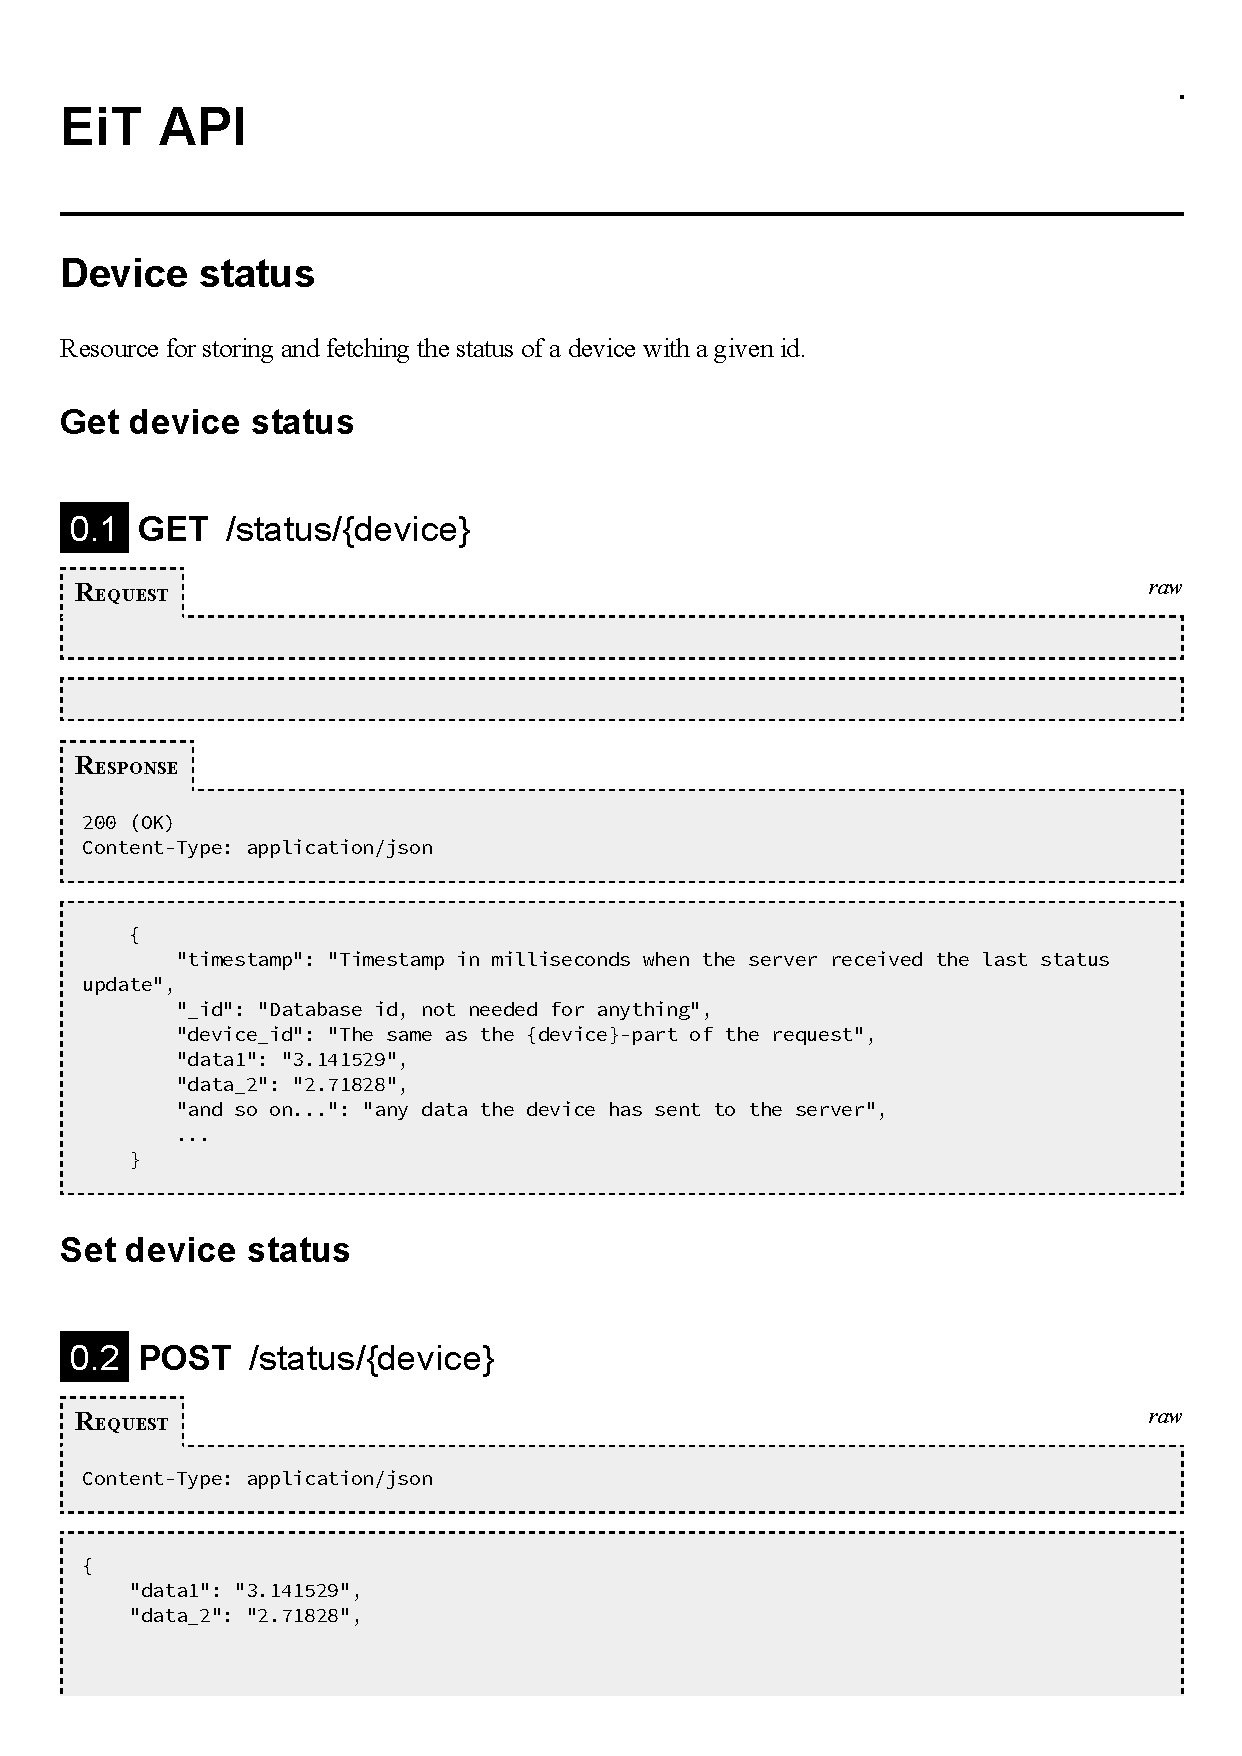
\includepdf[pages=-]{httpapi.pdf}

\chapter{Agent code}

\section{car.h}
\lstinputlisting[language=C++]{include/car.h}
\section{car.cpp}
\lstinputlisting[language=C++]{src/car.cpp}

\section{motor.h}
\lstinputlisting[language=C++]{include/motor.h}
\section{motor.cpp}
\lstinputlisting[language=C++]{src/motor.cpp}

\section{manipulator.h}
\lstinputlisting[language=C++]{include/manipulator.h}
\section{manipulator.cpp}
\lstinputlisting[language=C++]{src/manipulator.cpp}

\section{sensor.h}
\lstinputlisting[language=C++]{include/sensor.h}
\section{sensor.cpp}
\lstinputlisting[language=C++]{src/sensor.cpp}

\section{interface.h}
\lstinputlisting[language=C++]{include/interface.h}
\section{interface.cpp}
\lstinputlisting[language=C++]{src/interface.cpp}

\section{dynamixel.h}
\lstinputlisting[language=C++]{include/dynamixel.h}
\section{dynamixel.c}
\lstinputlisting[language=C++]{src/dynamixel.c}

\section{dxl\_ hal.h}
\lstinputlisting[language=C++]{src/dxl_hal.h}
\section{dxl\_ hal.c}
\lstinputlisting[language=C++]{src/dxl_hal.c}

\section{communication.h}
\lstinputlisting[language=C++]{include/communication.h}
\section{communication.cpp}
\lstinputlisting[language=C++]{src/communication.cpp}

\section{json\_ processing.h}
\lstinputlisting[language=C++]{include/json_processing.h}
\section{json\_ processing.cpp}
\lstinputlisting[language=C++]{src/json_processing.cpp}

\section{http\_ functions.h}
\lstinputlisting[language=C++]{include/http_functions.h}
\section{http\_ functions.cpp}
\lstinputlisting[language=C++]{src/http_functions.cpp}




\chapter{Example code}

\section{Car}
\lstinputlisting[language=C++]{example/Car/src/main.cpp}

\section{Interface}
\lstinputlisting[language=C++]{example/Interface/src/main.cpp}

\section{Main}
\lstinputlisting[language=C++]{example/Main/src/main.cpp}

\section{Manipulator}
\lstinputlisting[language=C++]{example/Manipulator/src/main.cpp}

\section{Motor}
\lstinputlisting[language=C++]{example/Motor/src/main.cpp}

\section{ReadWrite}
\lstinputlisting[language=C++]{example/ReadWrite/ReadWrite.c}

\section{Sensor}
\lstinputlisting[language=C++]{example/Sensor/src/main.cpp}

\section{SyncWrite}
\lstinputlisting[language=C++]{example/SyncWrite/SyncWrite.c}

\chapter{Server code}

\section{Installation notes}
\lstinputlisting{server/INSTALL}

\section{Utility functions}
\lstinputlisting[language=Python]{server/tools/decorators.py}
\lstinputlisting[language=Python]{server/tools/helpers.py}

\section{Server logic}
\lstinputlisting[language=Python]{server/resources.py}

\section{Main program}
\lstinputlisting[language=Python]{server/server.py}

\chapter{Datasheets}
\section{AX-12}
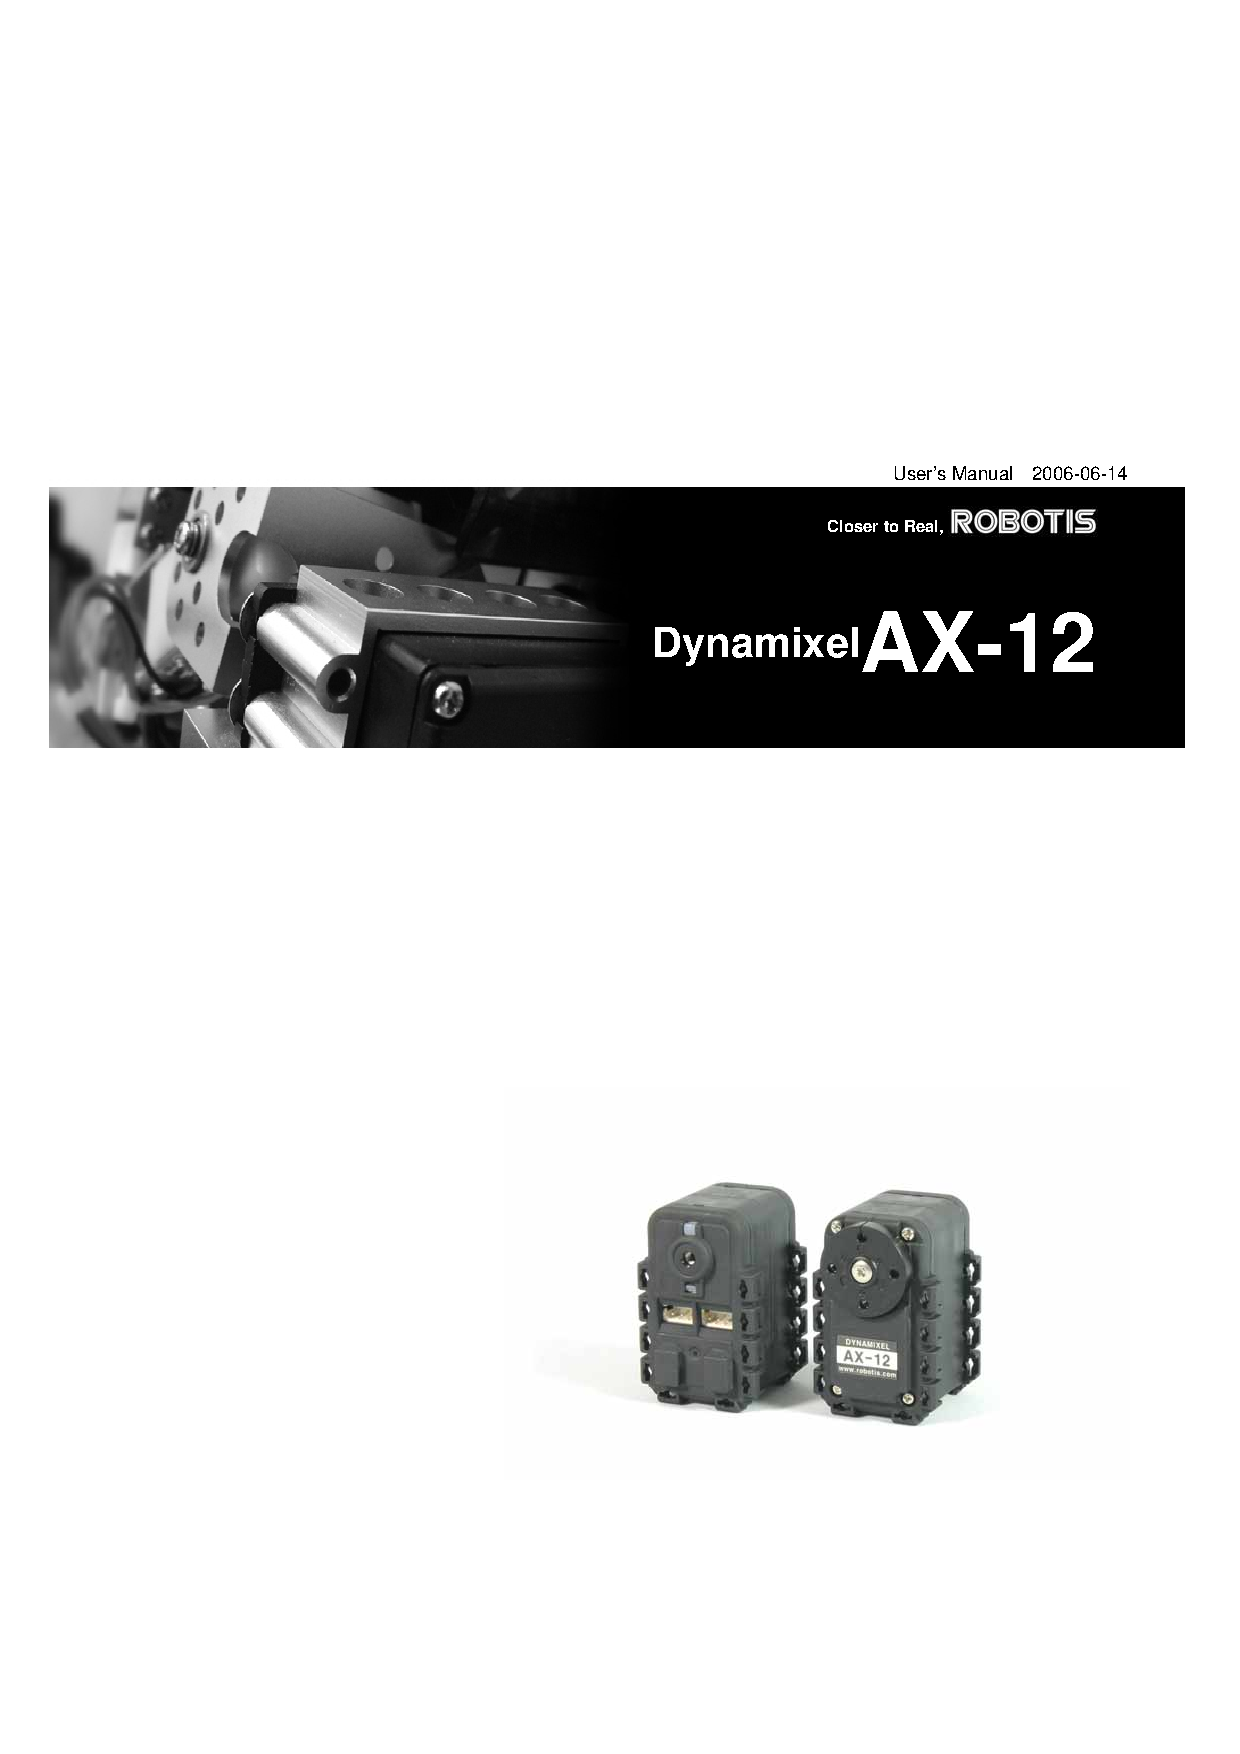
\includepdf[pages=-]{AX-12_Datasheet.pdf}
\section{AX-S1}
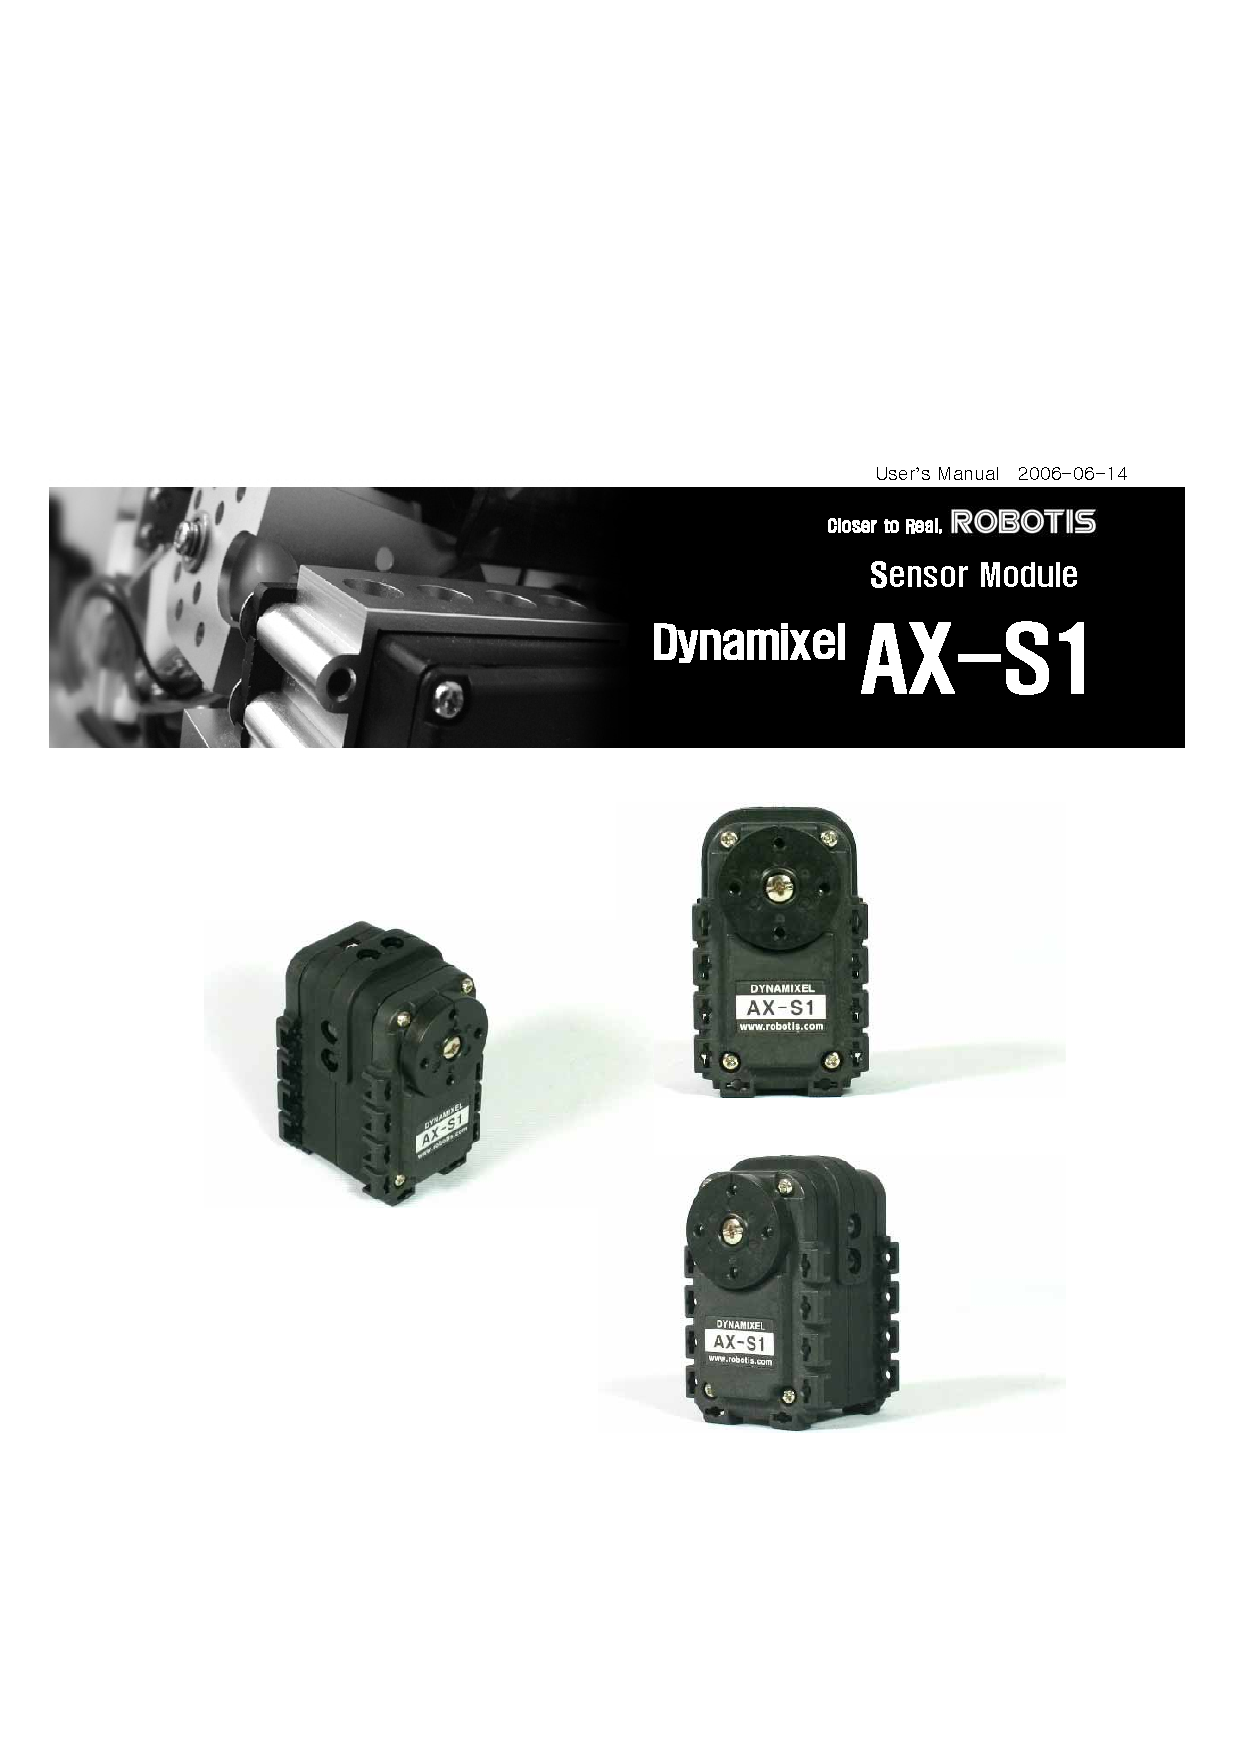
\includepdf[pages=-]{AX-S1_Datasheet.pdf}

\end{document}
